\documentclass[10pt]{article}
% RATISS Labs — shared preamble (Tectonic / LaTeX)
\usepackage[a4paper,margin=2.3cm]{geometry}
\usepackage{xcolor}
\usepackage{graphicx}
\usepackage{booktabs}
\usepackage{amsmath}
\usepackage{microtype}
\usepackage[hidelinks]{hyperref}
\definecolor{ratiss}{RGB}{14,107,102}
\definecolor{ratisslight}{RGB}{238,252,249}
\definecolor{inkgray}{RGB}{74,111,107}
\hypersetup{colorlinks=true,linkcolor=ratiss,urlcolor=ratiss,citecolor=ratiss}
\setlength{\parindent}{0pt}
\setlength{\parskip}{5pt}
\renewcommand{\familydefault}{\sfdefault}
\newcommand{\ratisshead}[4]{%
  {\color{ratiss}\rule{\linewidth}{1.2pt}}\vspace{6pt}\\
  {\LARGE\bfseries #1}\\[4pt]
  {\large #2}\\[2pt]
  {\color{inkgray}\small #3}\\[2pt]
  {\color{inkgray}\small #4}\vspace{8pt}\\
  {\color{ratiss}\rule{\linewidth}{0.6pt}}\vspace{10pt}%
}
\newcommand{\kwsection}[1]{\section*{\color{ratiss}#1}\addcontentsline{toc}{section}{#1}}
\newcommand{\sourcefoot}{%
  \vspace{10pt}{\color{ratiss}\rule{\linewidth}{0.6pt}}\vspace{4pt}\\
  {\color{inkgray}\scriptsize RATISS Labs --- independent, single-author laboratory, Yaoundé (Cameroon).
  No number in this document is invented: every value carries a source in
  Section~``Data and code availability'' or in the references.
  Negative results are published with the same prominence as positive ones.}%
}

\begin{document}
\ratisshead
{GHZ States on Real QPUs: an Ion / Superconducting Trilogy,\\ and a 97.27\% Four-Ion State}
{Jonathan Evina --- RATISS Labs, Yaoundé, Cameroon}
{Research object \texttt{ratiss-planck-002} · version v1 · 2026-09-30 · status: published}
{Hardware: Rigetti Cepheus-1-108Q, IQM Garnet, AQT IBEX Q1 via Open Quantum (attribution: www.openquantum.com/citation)}

\kwsection{Abstract}
Fourteen jobs were executed on 29/09/2026 on three real quantum processors.
The centerpiece is a four-qubit GHZ state on trapped ions (job \texttt{df23deac})
measured at 97.27\%, i.e.\ $(497+499)/1024$ shots. The GHZ-4 trilogy ranks
ions 97.3\% $>$ Garnet 94.6\% $>$ Cepheus 79.3\%. Bell states reach 99.61\% and
GHZ-7 90.04\% on IBEX; a twelve-qubit GHZ (``chat-12'') reaches 66.0\% on Garnet.
Measured costs are 1 / 2 / 15 Spark credits per 1024 shots for Cepheus / Garnet / IBEX.
The ion slope is compatible with $-1.9$ fidelity points per qubit, with local slopes
$-1.2$ then $-2.4$: a decay that accelerates.

\kwsection{Scientific question}
How does GHZ fidelity decay with qubit count, and how does that decay differ between
trapped-ion and superconducting modalities?

\kwsection{Method}
Multi-line QASM (\texttt{include "qelib1.inc";}), job subcategory \texttt{phys:oth},
quote approved only after reading the device quote line (``Auto-selected plan: N
credits''). Laboratory doctrine: one shot batch at a time, order Garnet $\rightarrow$
Cepheus $\rightarrow$ IBEX; never cancel a job without an explicit order; access tokens
have a $\approx$5 min TTL and are refreshed per call.

\begin{figure}[h]\centering
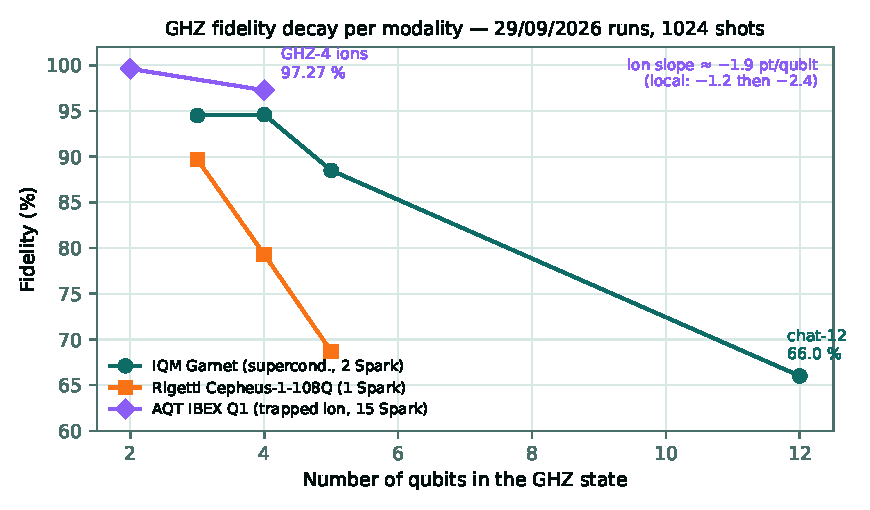
\includegraphics[width=0.95\linewidth]{fig/qpu-ghz-decay.pdf}
\caption{GHZ fidelity versus qubit count per modality (29/09/2026, 1024 shots).
Ion points: Bell 99.61\% (2q), GHZ-4 97.27\%. Garnet: 94.5 / 94.6 / 88.5 / 66.0\%.
Cepheus: 89.7 / 79.3 / 68.7\%.}\label{fig:decay}
\end{figure}

\kwsection{Results}
\begin{itemize}
  \item GHZ-4 trapped ions, \texttt{df23deac}: 97.27\% --- counts $0000=497$, $1111=499$ over 1024 shots.
  \item GHZ-4 trilogy: ions 97.3\% $>$ Garnet 94.6\% $>$ Cepheus 79.3\%.
  \item Bell 99.61\% and GHZ-7 90.04\% on IBEX Q1 (15 Spark each).
  \item Separated GHZ-3/4/5 on Garnet: 94.5 / 94.6 / 88.5\% (2 Spark); Cepheus trilogy 89.7 / 79.3 / 68.7\% (1 Spark).
  \item Chat-12 (GHZ-12, \texttt{b373d22f}): 66.0\% (2 Spark).
  \item Ion slope $\approx -1.9$ pt/qubit over three points (local slopes $-1.2$ then $-2.4$).
\end{itemize}
The raw counts of \texttt{df23deac} were re-downloaded and recomputed on 03/10/2026
from the signed output URL: 97.27\% confirmed identically.

\kwsection{Negative results}
\begin{itemize}
  \item Episodic-shot runs on co-hosted Garnet collapsed to 45\% vs 94\% $\rightarrow$
        RATISS law of the episodic shot: all-to-all ONLY on co-hosted devices.
  \item Job \texttt{407cd969} cancelled $\rightarrow$ 15 Spark refunded (first refund of the lab).
  \item Chat-12 at 66.0\%: below target, published as is.
\end{itemize}

\kwsection{Controls}
Quote read before approval; raw counts archived; server timestamps replayable.
Known SDK defect: \texttt{download\_job\_output} raises
\texttt{'str' object has no attribute 'output\_data\_url'} (still present in SDK 0.4.3);
harvesting uses \texttt{get\_job(...).output\_data\_url} instead.

\kwsection{Reproducibility}
Raw counts: \texttt{RATISS-PLANCK/resultats/qpu\_ghz4\_ibex\_counts.json};
register of the 14 jobs: \texttt{RATISS-ARCHIVES/preuves/qpu/openquantum-20260929.json}.

\kwsection{Limitations}
1024 shots: statistical uncertainty not reduced further (credit cost).
Cross-modality comparison is not at constant qubit count beyond the trilogy.

\kwsection{Data and code availability}
\url{https://github.com/jonathansearch/RATISS-PLANCK} (seal 52/52, MIT).
Platform attribution mandatory: www.openquantum.com/citation. Zenodo DOI: to be assigned.

\sourcefoot
\end{document}
